\section{Mean-field (deterministic) annealing} \label{sec:mean-determ-anne}

\mode<presentation>{
\begin{frame} 
    \begin{center} \huge
        \secname
    \end{center}
    \begin{center}
    Take simulated annealing \\
    but \\
		go faster, go deterministic
    \end{center}
\end{frame}
}

\begin{frame}{\secname}
 %\vspace{-2mm}
%\begin{block}{Simulated Annealing}
%\begin{itemize}
%\itr stochastic optimization: computationally expensive (sampling!)
%\itr stationary distribution $P_{(\vec{s})}$ known (for each $\beta_t$), why not evaluate?
%\itr but: maxima of $P_{(\vec{s})}$ equally hard to obtain as minima of $E_{(\vec{s})}$
%\itr moments? for $\beta \rightarrow \infty$: $\langle \vec{s} \rangle_P$ converges to $\vec{s}^*$ of minimal cost (caveat: true only if $P_{(\vec{s})}$ has only one global optimum)
%\itr but: moments of $P_{(\vec{s})}$ can -- in general -- not be calculated analytically
%\end{itemize}
%\end{block}
%\vspace{-2mm}
\slidesonly{
\begin{center}
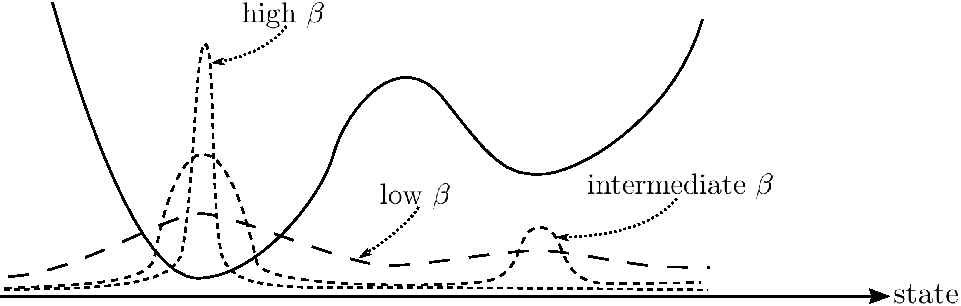
\includegraphics[width=12cm]{img/section3_fig7}  
\end{center}
}

\only<1>{

\begin{block}{Approximation by Mean-Field Annealing}
\begin{itemize}
\itR idea: approximate $P_{(\vec{s})}$ by a computationally tractable distribution $Q_{(\vec{s})}$
\itR this distribution is then used to calculate the first moment $\langle \vec{s} \rangle_Q$\\
\itR the first moment is tracked during the annealing schedule $\beta_t$
\itR hope: $\displaystyle \langle \vec{s} \rangle_Q \to $ $\vec{s}^*$ for $\beta_t\to\infty$
\end{itemize}
\end{block}

}

\only<2>{
\question{Why fixate on the first moment?}

\pause

- to localize the peak of the distribution as entropy decreases. 
At $\beta_t \rightarrow \infty$, the peak will have localized around the state where the cost is minimal, revealing the optimal state $\vec s^*$

}

\only<3>{

\question{Do we still need the annealing process?}

-Yes, because still need a tradeoff between exploration and exploitation.
}

 
\end{frame}

\subsection{Factorizing distribution}

\begin{frame}{\subsecname}
\begin{block}{Distribution $Q_{(\vec{s})}$ to approximate $P_{(\vec{s})}$}
\vspace{-0.35cm}
\begin{equation}
	Q_{(\vec{s})} \quad
= \quad \frac{1}{Z_Q} \exp \left\{ -\beta E_Q\right\} \quad
= \quad \frac{1}{Z_Q} \exp \Big\{ -\beta \sum\limits_{k}
		\underbrace{ e_k }_{ \text{parameters} } \mathrm{s}_k \Big\}
\end{equation}
\vspace{-0.65cm}
\begin{itemize}
 \item Gibbs distribution with costs $E_Q$ linear in the state variable $\vec{s}_k$
 \item factorizing distribution $Q_{(\vec{s})} = \Pi_k Q_k(s_k)$ with $Q_k(s_k) 
 = \frac{1}{Z_{Q_k}} \exp (-\beta e_k\mathrm{s}_k)$
% \end{itemize}
% \end{block}
% \vspace{-0.2cm}
% \begin{block}{Properties of $Q$}
% \begin{itemize}
 \item $Q_{(\vec{s})}$ factorizing $\iff s_k$ independent $\implies
    \langle \Pi_k s_k \rangle_Q = \Pi_k \langle s_k\rangle_Q
    \quad \!\! (\substack{\text{moments}  \\ \text{factorize}})$
 \item
 $ \big< s_k \big>_Q = \frac{\sum\limits_{s_k} s_k \exp(-\beta e_k s_k)}{
					\sum\limits_{s_k} \exp(-\beta e_k s_k)}$
\end{itemize}
\end{block}
% \vspace{-0.3cm}
\begin{itemize}
      \itr family of distributions parametrized by the \emph{mean fields} $e_k$
      \itr determine $e_k$ such that this approximation is as good as possible
\end{itemize}
\end{frame}


\begin{frame}{Mean-field approximation}
\begin{block}{Quantities}
\begin{equation}
	\begin{array}{llc}
	P_{(\vec{s})} 
	& = \frac{1}{Z_p} \exp(-\beta E_p) 
	& \substack{ \text{true distribution} } \\
	Q_{(\vec{s})} 
	& = \frac{1}{Z_Q} \exp\big(-\beta \overbrace{\sum\limits_k e_k s_k}^{E_Q} \big)
	& \substack{ \text{approximation: family of} \\ \text{factorizing distributions} } \\\\
	e_k:
	& \text{\textit{mean fields} }
	& \substack{ \text{parameters to} \\ \text{be determined} }
	\end{array}
\end{equation}
\end{block}
\begin{block}{Good approximation of $P$ by $Q$}
\vspace{0.1cm}
$\rightarrow$ minimization of the KL-divergence:
\begin{equation}
	\dkl(Q||P) = \sum\limits_{\vec{s}} Q_{(\vec{s})} \ln \frac{Q_{(\vec{s})}}{
		P_{(\vec{s})}} \eqexcl \min_{\vec{e}}
\end{equation}
\end{block}
\end{frame}

\subsubsection{Setting up the arguments for the KL divergence}

\begin{frame}{\subsubsecname}

Let $P$ be the reference distribution (target) and $Q$ be the parameterized distribution (what we tune).

\question{How do we generally decide between minimizing $\dkl(Q||P)$ vs. $\dkl(P||Q)$?}

\pause

-We look at what kind of solutions are found by each usage of the KL divergence:  


\end{frame}

\begin{frame}{\subsubsecname}

\begin{block}{minimizing forward $\dkl$}

\slidesonly{
\begingroup
\footnotesize
}
\begin{equation}
	\dkl(P||Q) = \sum\limits_{\vec{s}} P_{(\vec{s})} \ln \frac{P_{(\vec{s})}}{
		Q_{(\vec{s})}} \eqexcl \min_{\text{parameters}}
\end{equation}
\slidesonly{
\endgroup
}
\end{block}

\begin{itemize}
\item \notesonly{Corresponds to }the \emph{maximum-likelihood} solution\notesonly{ (will discuss later in density estimation)}
\item Seen in Infomax and density estimation.
\item Change $Q$ such that it ``covers'' as much of $P$ as possible.
\notesonly{\item If $P$ has two modes minimizing $\dkl(P||Q)$ will find a $Q$ that is wide enough to cover both.}
\end{itemize}

\pause

\begin{center}
	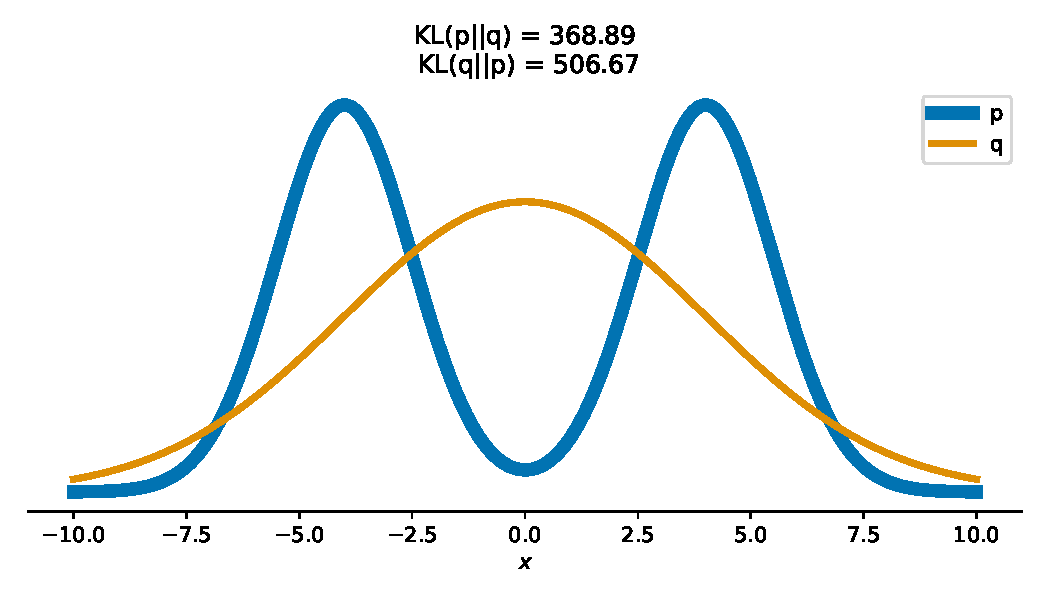
\includegraphics[width=0.55\textwidth]{img/kl_fwd}
\end{center}

\end{frame}

\begin{frame}{\subsubsecname}

\begin{block}{Reverse $\dkl$}
\slidesonly{
\begingroup
\footnotesize
}
\begin{equation}
	\dkl(Q||P) = \sum\limits_{\vec{s}} Q_{(\vec{s})} \ln \frac{Q_{(\vec{s})}}{
		P_{(\vec{s})}} \eqexcl \min_{\text{parameters}}
\end{equation}
\slidesonly{
\endgroup
}
\end{block}

\begin{itemize}
\item Corresponds to the \emph{maximum-entropy} solution.
\item With $Q$ in the numerator of the $\log$ we prefer solutions where $Q$ is zero even if $P$ is non-zero. 
\end{itemize}

\pause
\only<2>{
\slidesonly{
\begin{center}
	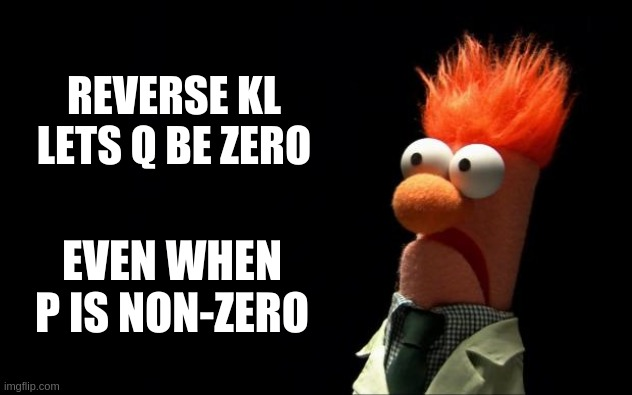
\includegraphics[width=0.3\textwidth]{img/meme_revkl}
\end{center}

}
}

\only<3>{

\begin{center}
	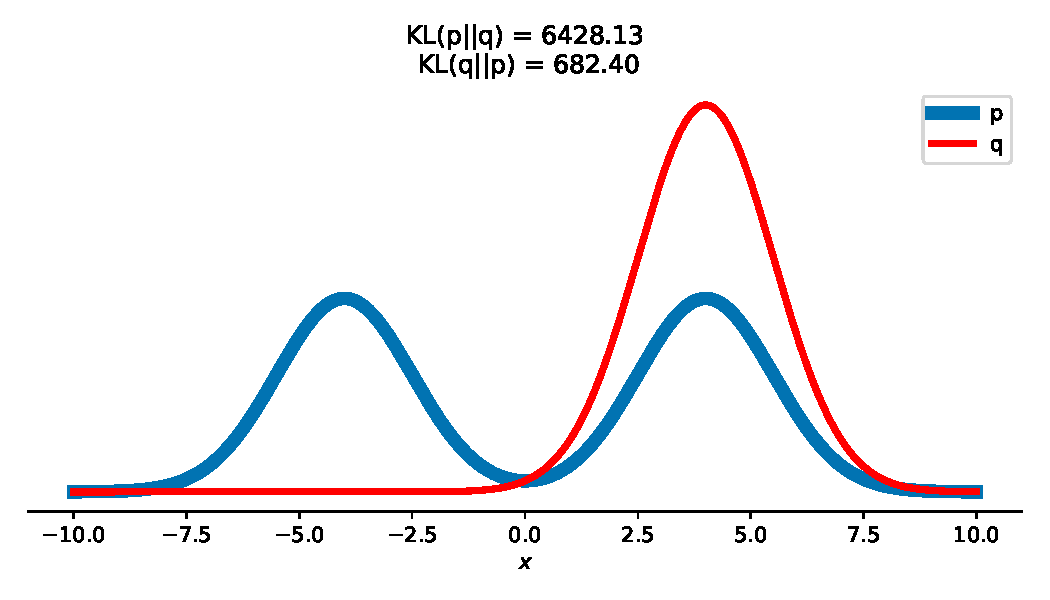
\includegraphics[width=0.55\textwidth]{img/kl_rev}
\end{center}

\notesonly{If $P$ has two modes a ``good'' $Q$ is one that fits one mode very well even if it completely ignores the other mode\footnote{Additional resources for explaining the differences between forward and reverse KL:\\ 
\href{https://dibyaghosh.com/blog/probability/kldivergence.html} \\ and \\
%\href{https://www.quora.com/What-is-the-theoretical-advantage-disadvantage-between-minimizing-KL-Q-P-and-KL-P-Q-in-Bayesian-variational-inference}
}.
}
}
\end{frame}

\begin{frame}

\question{Why minimize the reverse $\dkl$ for mean-field approximation?}

\slidesonly{
\begin{equation}
	\dkl(Q||P) = \sum\limits_{\vec{s}} Q_{(\vec{s})} \ln \frac{Q_{(\vec{s})}}{
		P_{(\vec{s})}} \eqexcl \min_{\vec{e}}
\end{equation}
}

- Even if our assumption about $P$ having a single moment is wrong. If it has two minima, picking one is better than picking a solution in the middle.

\end{frame}

\subsubsection{Mean-Field annealing for Ising model}

\begin{frame}{Mean-field annealing\only<2>{~ for Ising model}}
\begin{block}{Algorithm}
% \begin{algorithm}[h]
%   \DontPrintSemicolon
%   initialization: $\langle \vec{s} \rangle_0, \beta_0, t = 0$ \;
%   \Begin(Annealing loop){ 
%     \Repeat{$|e_k^\mathrm{old}-e_k^\mathrm{new}| < \varepsilon$}
%     {
%       calculate mean-fields: $e_k, \ \ k = 1, \ldots, N$ \;
%       calculate moments: $\big<s_k\big>_Q,\ \ k = 1, \ldots, N$ \;
%     }
%     increase $\beta$ \;
%     }
%   \end{algorithm}
% 

\texttt{initialization:} $\langle \vec{s} \rangle_0, \beta_0$ \; \\
\texttt{BEGIN Annealing loop}\\
\oident \texttt{Repeat} \\
\begin{itemize}
  \item calculate mean-fields: $e_k\visible<2>{= - \sum\limits_{\substack{i=1 \\ i\ne k}}^N W_{ik} \langle s_i \rangle_Q}, \ \ k = 1, \ldots, N$ \;
  \item calculate moments: $\big<s_k\big>_Q\visible<2>{= \tanh(-\beta e_k)},\ \ k = 1, \ldots, N$ \;
\end{itemize}
\oident\texttt{Until $|e_k^\mathrm{old}-e_k^\mathrm{new}| < \varepsilon$} \\
\oident increase $\beta$ \; \\
\texttt{END Annealing loop}
\end{block}
\end{frame}

\begin{frame}
\slidesonly{
\begin{center}
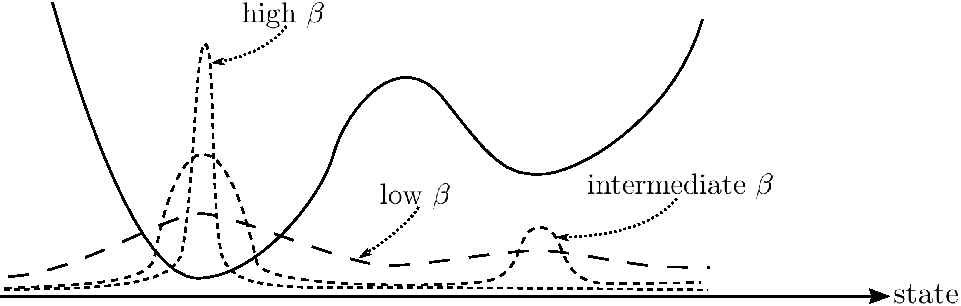
\includegraphics[width=12cm]{img/section3_fig7}  
\end{center}
}
\end{frame}
